\apendice{Plan de Proyecto Software}\label{anex:A}

\section{Introducción}

%Ref david goo bees https://github.com/davidmigloz/go-bees puede ayudar con la memoria
Una de las actividades de un proyecto software es la fase de planificación. En esta fase se estima el esfuerzo, el tiempo y el dinero que se espera invertir en el proyecto. El objetivo principal de la fase de planificación es estimar si se puede realizar el proyecto con éxito y, en ese caso, tener una guía de referencia para el proceso de desarrollo. Este anexo recoge los documentos generados en este proceso y se divide en dos partes:
\begin{description}
	\tightlist
	\item[Planificación temporal.] En esta parte se estima el tiempo y el esfuerzo que se requieren para la realización del proyecto.
	\item[Estudio de la viabilidad.] Esta parte se estima si el proyecto es viable tanto económica como legalmente, por tanto se dividirá en dos secciones:
	\begin{description}
		\tightlist
		\item[Viabilidad económica.] Análisis del coste y del beneficio que supondría la realización del proyecto.
		\item[Viabilidad legal.] Análisis de las leyes que se aplicarían desde el comienzo del proyecto. En un proyecto software tienen especial importancia las licencias y la Ley de Protección de Datos.
	\end{description}
\end{description}

\section{Planificación temporal}
No se ha realizado una planificación temporal del proyecto. Se han seguido los 12 principios del manifiesto ágil y el modelo SCRUM \cite{noauthor_scrum_2019}:
\begin{itemize}
	\tightlist
	\item Se ha aplicado un desarrollo incremental y evolutivo.
	\item Se han realizado iteraciones (\textit{sprints}) de dos semanas. Al finalizar un sprint se realizaba una reunión entre el tutor y el alumno que daba comienzo al siguiente sprint y que consta de dos partes:
	\begin{itemize}
		\item Una parte de revisión del sprint en la que se exponía una parte operativa del producto realizada durante el sprint.
		\item Otra de planificación del siguiente sprint en la que se determinaba el trabajo y los objetivos a alcanzar durante el siguiente sprint. Esto quedaba reflejado como una pila de tareas que se debían completar durante el sprint y que han sido registradas en el sistema de gestión de incidencias de GitLab.
	\end{itemize}
\end{itemize}
\subsection{Sprints}
A continuación se definen los sprints y sus respectivas pilas de tareas que se llevaron a cabo durante la realización del proyecto. 

Según la naturaleza de los sprints, en el proceso del desarrollo se pueden diferenciar varias etapas:
\begin{itemize}
	\item  Una primera etapa de \textbf{investigación} de las herramientas que se utilizarán durante el proceso y de \textbf{configuración} del entorno de desarrollo.
	\item En la segunda etapa se aprecian tareas de \textbf{diseño} de la parte lógica de la aplicación. Se diseña el framework de conexión a forjas de repositorios, se implementa el framework descrito en \textit{Soporte de Métricas con Independencia del Lenguaje para la Inferencia de Refactorizaciones}  \cite{marticorena_soporte_2005} para el cálculo de métricas y se diseñan los modelos de datos que serán utilizados por la aplicación.
	\item Durante la segunda etapa se apreció que se debía facilitar el \textbf{flujo de trabajo}, la comunicación entre tutor y alumno y facilitar las reuniones de revisión y planificación del sprint.
	\item Etapa  de diseño e implementación de la \textbf{interfaz gráfica} y \textbf{mejora de características} que precisaban de cambios en la parte lógica de la aplicación que se diseñó en la segunda etapa.
	\item Etapa de \textbf{documentación} en la que se escribe la memoria y los anexos. También se preparan videotutoriales y manuales de usuario.
\end{itemize}

\subsubsection{Investigación y configuración}

Los dos primeros sprints estuvieron dedicados a la investigación de herramientas y configuración del entorno de desarrollo. Por cada sprint se observa en la Fig. \ref{fig:AnexA_Sprints_1_EstudioYConfig} su descripción, la fecha de apertura y cierre, y el número de issues asociadas. Y en la Fig. \ref{fig:AnexA_Issues_1_EstudioYConfig} se muestran las descripciones de las primeras tareas que se definieron, la mayoría etiquetadas como `\textit{Research}' (Estudio o investigación) y `\textit{Project Configuration}' (Configuración del proyecto). En la Fig. \ref{fig:AnexA_Sprints_1_EstudioYConfig_BurnDown} se muestra un gráfico \textit{burndown} \footnote{Gráfico de trabajo pendiente. En él se muestran las issues abiertas en el ciclo de vida del sprint} del segundo sprint, ya que del primero no hay sido posible obtenerlo debido a que GitLab no lo ha podido generar seguramente por una mala gestión de las issues.

\begin{figure}[!h]
	\centering
	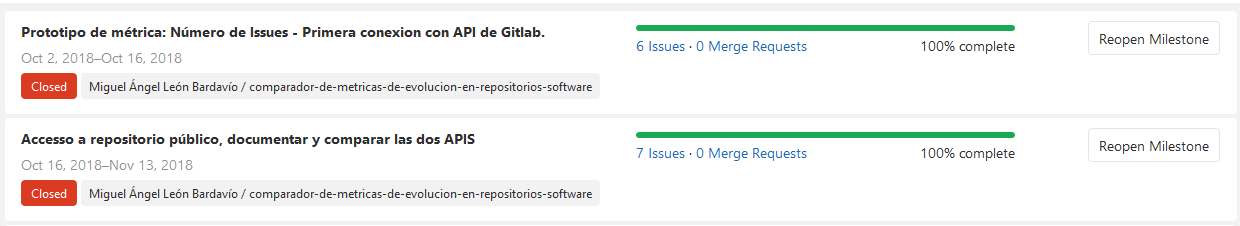
\includegraphics[scale=0.40]{AnexA_Sprints_1_EstudioYConfig}
	\caption{Sprints iniciales del proyecto en GitLab.}
	\label{fig:AnexA_Sprints_1_EstudioYConfig}
\end{figure}
\FloatBarrier

\begin{figure}[!h]
	\centering
	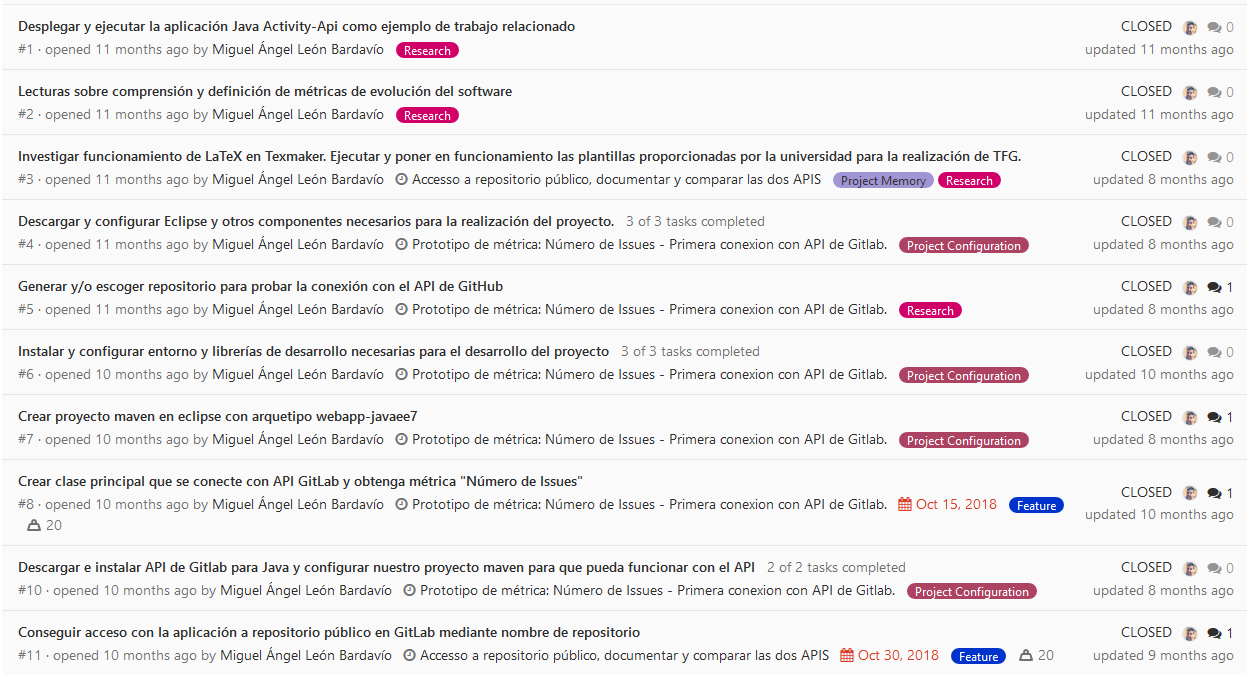
\includegraphics[scale=0.40]{AnexA_Issues_1_EstudioYConfig}
	\caption{Primeras issues del proyecto, la mayoría etiquetadas como `Research' o `Project Configuration'}
	\label{fig:AnexA_Issues_1_EstudioYConfig}
\end{figure}
\FloatBarrier

\begin{figure}[!h]
	\centering
	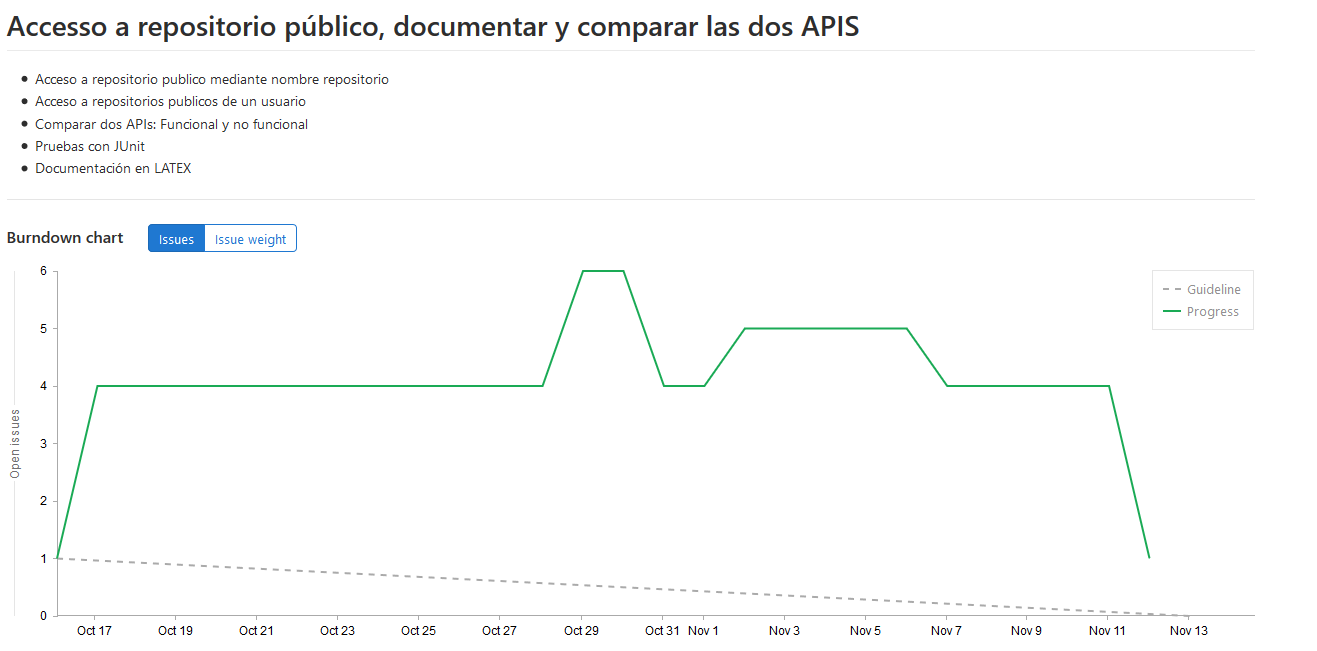
\includegraphics[scale=0.40]{AnexA_Sprints_1_EstudioYConfig_BurnDown}
	\caption{Gráfico burndown del segundo sprint Acceso a repositorio público, documentar y comparar las dos APIS}
	\label{fig:AnexA_Sprints_1_EstudioYConfig_BurnDown}
\end{figure}
\FloatBarrier

Esta etapa de investigación y configuración duró un mes (dos sprints) y sus decisiones afectaron a todo el proyecto. Se recopiló información sobre trabajos relacionados como \textit{Activiti-Api} \cite{rlp0019_software_2019}, \textit{Soporte de Métricas con Independencia del Lenguaje para la Inferencia de Refactorizaciones}  \cite{marticorena_soporte_2005} y \textit{sPACE: Software Project Assessment in the Course of Evolution} \cite{ratzinger_space:_2007} y se estudió los entornos y herramientas que se utilizarían para el desarrollo del proyecto.

\subsubsection{Diseño e implementación}

Después de esta etapa de investigación, comenzó una etapa de diseño. En esta etapa, las tareas que se definen se relacionan con el diseño de la parte lógica del sistema software a construir, se comienza con la implementación y se empiezan a utilizar las herramientas investigadas anteriormente para construir el sistema. 

Esta etapa de diseño tuvo duración de 3 sprints y uno extra para la configuración del flujo de trabajo que se explica en el siguiente apartado. Esto se puede apreciar en la Fig.  que muestra los sprints relacionados a esta etapa y en la Fig. que muestra las issues relacionadas con la etapa de diseño. La mayoría de estas issues cuentan con la etiqueta `\textit{Design}'.

\subsubsection{Configuración del flujo de trabajo}

Dentro de la fase de diseño se decidió dedicar un tiempo a un tipo de configuración del proyecto que facilitaría el flujo de trabajo y las reuniones de revisión/planificación del sprint. Las principales tareas para mejorar el flujo de trabajo fueron:
\begin{itemize}
	\item Configurar la gestión del proyecto con Maven
	\item Configurar los procesos de integración y despliegue continuo con GitLab (CI/CD)
	\item Realizar pruebas unitarias con JUnit y automatizar su ejecución gracias a Maven y los \textit{pipelines} (CI/CD) de GitLab .
	\item Configurar revisiones automáticas de calidad y de cobertura de las pruebas gracias a Codacy, Jacoco y GitLab.
	\item Configurar un entorno en Heroku donde poder desplegar la aplicación y así poder ser revisada por el tutor fácilmente.
	\item Configurar badges \footnote{Son placas que aportan información rápida sobre el estado del proyecto en ciertos aspectos como la cobertura, la calidad de código o el estado del proceso de CI/CD} para representar los el estado de la calidad de código, cobertura, despliegue y los trabajos de CI/CD.
\end{itemize}

Esta fase duro un sprint y comenzó antes de terminar la fase de diseño, como se observa en la Fig. en un milestone con título ``Excepciones, log, test, pom y CI''. Las issues que se definieron se caracterizan por tener las etiquetas `\textit{Test}', `\textit{Project Configuration}' o `\textit{Question}', como se puede observar en la Fig. . También se muestra en la Fig. un gráfico burndown del sprint.

\subsubsection{Implementación de la interfaz gráfica y mejora de las catacterísticas}
Es la etapa más extensa, duró 8 sprints que se muestran en la Fig. . Esta etapa comienza con un estudio de la herramienta Vaadin para crear la interfaz gráfica y la viabilidad de su uso en el proyecto. Para ello, se realizaron varias pruebas de integración con el entorno de desarrollo (Versión de Java, Eclipse, Maven, etc), se realizó un primer prototipo sencillo y se comprobó que se podría hacer una interfaz gráfica con la licencia gratuita. Una vez terminado con éxito estas pruebas de viabilidad, comenzó el desarrollo de la interfaz gráfica del proyecto.

La interfaz gráfica da un aspecto más visible de lo que el proyecto podría llegar a ser. Los requisitos funcionales evolucionaban conforme evolucionaba la interfaz. Por ejemplo, se decidió agregar varias formas de añadir un repositorio o añadir más formas de conectarse a GitLab.

En la Fig. se muestran las primeras tareas de esta etapa. Destacan por ser etiquetadas con `GUI' y `Feature'.

Se muestra en la Fig. los gráficos burndown de esta fase.


\subsubsection{Documentación}
Esta etapa comenzó al terminar el desarrollo del proyecto. En esta se realiza la memoria y los anexos del proyecto, así como videotutoriales u otros manuales de usuario. Esta fase duró 2 sprints (ver Fig. ) y sus tareas son etiquetadas todas con `Project Memory' (ver Fig. ). En la Fig. se muestran los gráficos burndown del sprint.

\section{Estudio de viabilidad}
\subsection{Viabilidad económica}
En esta sección se realiza un análisis coste-beneficio del proyecto.

\subsection{Viabilidad legal}
En esta sección se realiza un estudio de las leyes que se aplican a este proyecto para asegurar que la realización del proyecto no supondrá ninguna violación de estas leyes. 



